% =============================================================================
% SECURITY ANALYSIS — the keystone chapter that makes this a cryptographic thesis.
% Canonical crypto spine: Preliminaries -> Construction -> SECURITY -> Evaluation.
% Builds ONLY on what is already established: §3 BDEC security experiments
% (EUF-CMA / anonymity / unlinkability) and §5's precompile-soundness argument.
% Assumptions are folded into the theorem hypotheses and discussed in prose,
% in the manner of the cited literature, not enumerated as a graded ledger.
% Honesty bar = Sako; proof-checker posture.
% =============================================================================

\section{Security Analysis}\label{sec:security}

Section~\ref{sec:system} described an instrument: a precompile suite that moves
PLUM's dominant field operations out of emulated guest code, together with a
RISC~Zero and SP1 realisation of the BDEC credential-generation relation. A
performance instrument is meaningful for a credential system only if it does not
silently weaken the security the system provides. This section makes that
requirement precise. We fix the security model and threat model in
Section~\ref{ssec:threat-model}, prove in Section~\ref{ssec:preservation} a
preservation theorem that bounds how far the move to a zkVM substrate and the
precompile suite can shift the adversary's advantage in each of BDEC's security
experiments, and then isolate in Section~\ref{ssec:zk-gap} the one property the
analysis does not deliver on consumer hardware, namely zero-knowledge, and hence
anonymity, of the proof actually produced. This last point follows from how the
toolchain produces proofs and not from any weakness in the construction itself,
so we treat it as a finding about the substrate.

\subsection{Security Model and Threat Model}\label{ssec:threat-model}

BDEC is proved secure in three experiments, formalised in
Section~\ref{sec:prelim}. Unforgeability requires that an adversary with
issuance and showing oracles cannot produce an accepting showing for a statement
outside its honestly issued set, beyond negligible advantage. Anonymity and
unlinkability are challenge-bit experiments in which the adversary cannot
distinguish, beyond advantage $|\Pr[b'=b]-\tfrac12|$, which of two honestly
issued credentials produced a challenge showing (anonymity) or which of two
pseudonym keys issued a single challenge credential (unlinkability). We write
$\mathsf{Adv}^{\mathsf{unf}}_{\AC}$, $\mathsf{Adv}^{\mathsf{anon}}_{\AC}$, and
$\mathsf{Adv}^{\mathsf{unlink}}_{\AC}$ for the respective advantages, all defined
in Section~\ref{sec:prelim}.
\begin{definition}[zkVM-BDEC advantage]\label{def:zkvm-bdec-adv}
For $\bullet\in\{\mathsf{unf},\mathsf{anon},\mathsf{unlink}\}$, write
$\mathsf{Adv}^{\bullet}_{\mathsf{zkVM\text{-}BDEC}}(\mathcal A)$ for the advantage
$\mathsf{Adv}^{\bullet}_{\AC}(\mathcal A)$ of Section~\ref{sec:prelim} evaluated on
the BDEC scheme instantiated with PLUM as the signature scheme $\Sig$ and the zkVM
as the zkSNARK $\Pi$.
\end{definition} BDEC's Theorems~1
through~3~\cite{10.1007/978-981-96-0957-4_3} already prove these properties, so
this section does not re-prove them. It bounds how far the move to a zkVM
substrate shifts each advantage.

The parties are the teaching authorities and the issuer, who hold signing keys,
together with the holder and the relying party. The ledger roots
$\mathsf{rt}_{\mathsf{cred},e}$, $\mathsf{rt}_{TA,e}$, and $\mathsf{rt}_{\RL,e}$
are public and authenticated. The prover is the holder generating a showing, and
the verifier is the relying party, which chooses the presentation predicate
$\phi$ at presentation time. The adversary is the standard anonymous-credential
adversary of Section~\ref{sec:prelim}, lifted to the zkVM execution setting: it
may request issuance of credentials on attribute vectors of its choice, observe
showings produced by honest holders, act as a malicious verifier choosing $\phi$
adaptively, and act as a malicious prover attempting to produce an accepting
showing it should not be able to prove. Following PLUM, the unforgeability we
inherit is established against classical adversaries in the classical
random-oracle model. Its post-quantum reading rests on the underlying
power-residue PRF and collision-resistance assumptions being quantum-hard,
whereas the lift of the EU-CMA reduction itself to the quantum random-oracle
model is a separate question that PLUM does not settle and that we do not
re-establish here. That such a lift is \emph{attainable} for this PRF family is
shown by Pegasus~\cite{cryptoeprint:2025/1841}, which proves {(Q)ROM} security for
a power-residue-PRF signature; Pegasus is a different construction (a
commit-and-open $\Sigma$-protocol, not PLUM's STIR-based design), so it does not
close PLUM's own lift but it removes any presumption that the PRF family itself
is the obstacle.

Side-channel and timing attacks on the prover host, denial of service, and the
physical security of signing keys are out of scope, since they are orthogonal to
the substrate question this thesis studies. The trusted computing base of the
zkVM regime is the RISC-V execution circuit, the precompile chips, and the
lookup argument that binds them to the main execution trace.

The preservation theorem of Section~\ref{ssec:preservation} and the
precompile-soundness theorem of Section~\ref{sec:system} rest on four named
premises, each also stated inline where it is used. Premise~(T1), that the
cross-table lookup argument binds the precompile chips to the execution trace, is
assumed from the SP1 and RISC~Zero implementations (their logarithmic-derivative
lookup arguments~\cite{haback2022logup}), not independently verified here. Premise~(T2), that the
Griffin-$\mathbb{F}_p^{192}$ AIR admits only the reference permutation,
equivalently that $\epsilon_{\mathrm{AIR}}$ is negligible, is open: it is argued and
empirically supported in Appendix~\ref{app:proofs} but not established at the
constraint level. Premise~(T3), that PLUM's EU-CMA reduction treats Griffin and
field multiplication as black-box input--output maps, is argued from the structure
of that reduction. Premise~(T4), that PLUM admits a signature-transcript simulator,
equivalently that $\epsilon_{\mathrm{sZK}}$ is negligible, is open and is required
only by the anonymity and unlinkability bounds, PLUM's analysis establishing
EU-CMA security but not simulatability. The zkVM is additionally assumed
knowledge-sound and the modular-multiplication precompile sound, the latter
established for SP1 (\S\ref{ssec:bigint}) and cited for RISC~Zero; the
quantum-random-oracle lift of PLUM's EU-CMA reduction and of the nested
Fiat--Shamir transform is open, the analysis being in the classical
random-oracle model.

\subsection{Security Preservation}\label{ssec:preservation}

The analysis rests on one structural observation. The zkVM regime changes how
the BDEC relation $R_{\mathsf{show}}^{\Sig}$ (and the structurally analogous
credential-generation relation $R_{\mathsf{cre}}^{\Sig}$) is proved; the relation
itself, what it states, is unchanged. The relation
is fixed in Section~\ref{sec:prelim}, and both the static-circuit and the zkVM
regimes are proof systems for that same relation. Preservation therefore reduces
to two claims: that the substrate computes the same relation, and that its proof
system supplies the soundness and zero-knowledge that BDEC's reductions consume.
We treat the two in turn.

\begin{lemma}[Relation preservation]\label{lem:relation-preserve}
Suppose the host modular-multiplication precompile is sound, the cross-table
lookup argument binds the precompile tables to the main execution trace, the
zkVM is a knowledge-sound argument of knowledge for RISC-V execution, and the
Griffin-$\mathbb{F}_p^{192}$ AIR admits only the reference permutation. Then the
zkVM guest program with the precompile suite active accepts a pair $(x,w)$ if and
only if $R^{\Sig}(x;w)=1$, where $R^{\Sig}$ denotes either of the BDEC relations $R^{\Sig}_{\mathsf{cre}},R^{\Sig}_{\mathsf{show}}$ of
Section~\ref{sec:prelim}. The lemma is stated at the level of the intended guest
\emph{specification}; the code-level claim additionally requires that the zkVM
journal be bound to the public statement $x$, which the current RISC~Zero
prototype does not yet implement (Section~\ref{sec:system}). Absent that
binding, an accepting receipt does not certify which statement was evaluated, so
the code-level reading of the lemma is conditional on the journal fix.
\end{lemma}

\begin{proof}[Proof sketch]
A guest evaluation of the BDEC relations invokes only large-field multiplications
and Griffin permutations, which the precompiles return identically under the
lookup binding, together with native control flow covered by the zkVM's
knowledge-soundness; composing these per-operation equalities along the finite,
input-fixed execution yields equality of the accept-or-reject decision at the
program level. The Griffin step's constraint-level soundness rests on the AIR
argument of Appendix~\ref{app:proofs}, so the equality holds modulo premise~(T2);
the $9.4\times10^{9}$-cycle execute-mode run confirms the guest program's I/O but
does not exercise the AIR constraints. The step-by-step argument, including the
$k+2$ presentation predicates, is given in Appendix~\ref{app:preservation}.
\end{proof}

\begin{theorem}[Security preservation, conditional; classical ROM]\label{thm:security-preserve}
Suppose PLUM is EU-CMA secure in the classical random-oracle model and, for the
anonymity and unlinkability bounds only, additionally admits a signature-transcript
simulator with error $\epsilon_{\mathrm{sZK}}$ (premise~(T4), an \emph{open} premise
parallel to (T2): PLUM's analysis establishes only EU-CMA, whereas BDEC's
Theorems~2--3 simulate the credential and pseudonym transcripts with the signature's
own simulator). Suppose the zkVM is a
knowledge-sound argument of knowledge for RISC-V execution, the host
modular-multiplication precompile is sound, and the cross-table lookup argument
binds the precompile tables to the trace. Suppose further, as premise~(T3), that
PLUM's EU-CMA reduction treats Griffin and field multiplication as black-box
input--output maps, so that the precompile substitution leaves that reduction
unchanged. Suppose further, as an unverified
premise (T2), that the Griffin-$\mathbb{F}_p^{192}$ AIR admits only the reference
permutation; this premise is argued in Appendix~\ref{app:proofs} but not
established at the constraint level (see the discussion after the proof). Then for
every classical adversary $\mathcal{A}$ against the PLUM-instantiated,
zkVM-executed BDEC system, in the random-oracle model, the advantage is bounded by
five leaf errors: $\epsilon_{\mathrm{EUF}}$ (PLUM's EU-CMA error), $\epsilon_{\mathrm{KS}}$
(the zkVM argument's knowledge-soundness error), $\epsilon_{\mathrm{AIR}}$ (the
Griffin-AIR constraint-level soundness error), $\epsilon_{\mathrm{ZK}}$ (the produced
proof's zero-knowledge error), and $\epsilon_{\mathrm{sZK}}$ (PLUM's
signature-transcript-simulation error):
\begin{align}
  \mathsf{Adv}^{\mathsf{unf}}_{\mathsf{zkVM\text{-}BDEC}}(\mathcal{A})
  &\le \epsilon_{\mathrm{EUF}} + \epsilon_{\mathrm{KS}} + \epsilon_{\mathrm{AIR}},
  \label{eq:adv-unf}\\
  \mathsf{Adv}^{\mathsf{anon}}_{\mathsf{zkVM\text{-}BDEC}}(\mathcal{A})
  &\le \epsilon_{\mathrm{ZK}} + \epsilon_{\mathrm{sZK}},
  \label{eq:adv-anon}
\end{align}
and the same bound $\epsilon_{\mathrm{ZK}}+\epsilon_{\mathrm{sZK}}$ holds for unlinkability, whose game (BDEC Theorem~3) forwards a single challenge credential, so the one-transcript simulation applies once. These three bounds re-instantiate BDEC's Theorems~1--3~\cite{10.1007/978-981-96-0957-4_3} with PLUM as the signature scheme and the zkVM as the zkSNARK, expressed directly in the leaf errors below. The
term $\epsilon_{\mathrm{AIR}}$ is the AIR's constraint-level soundness error: the
probability, over the prover-chosen trace and the argument's verifier randomness,
that the argument accepts a trace whose Griffin transition differs from the
reference permutation. Premise~(T2) is the open, empirically-supported
claim (Appendix~\ref{app:proofs}) that $\epsilon_{\mathrm{AIR}}$ is negligible.
$\epsilon_{\mathrm{KS}}$ is the
knowledge-soundness error of the zkVM argument, $\epsilon_{\mathrm{EUF}}$ is the
EU-CMA error of PLUM (\cite[Theorem~1]{10.1007/978-981-95-2961-2_6}, carried over from Loquat's reduction~\cite{cryptoeprint:2024/868}), $\epsilon_{\mathrm{ZK}}$ is the zero-knowledge error of
the produced proof, and $\epsilon_{\mathrm{sZK}}$ is the signature-transcript
simulation error of PLUM (premise~(T4)), required because BDEC's anonymity and
unlinkability reductions simulate the credential and pseudonym transcripts with the
signature's own simulator (Theorems~2--3~\cite{10.1007/978-981-96-0957-4_3}), not
only the proof simulator.
\end{theorem}

\begin{proof}[Proof sketch]
By Lemma~\ref{lem:relation-preserve} the zkVM proves the same relation as BDEC's
static circuit, so we re-instantiate BDEC's three reductions with PLUM as the
signature scheme and the zkVM as the zkSNARK; all bounds are for classical
$\mathcal A$ in the random-oracle model. For \emph{unforgeability}, the zkVM
knowledge extractor recovers a witness from an accepting showing (cost
$\epsilon_{\mathrm{KS}}$); a malformed Griffin trace that passes the precompile
costs $\epsilon_{\mathrm{AIR}}$ (premise~(T2)); the recovered signature is then a
PLUM EU-CMA forgery (cost $\epsilon_{\mathrm{EUF}}$), giving~\eqref{eq:adv-unf}.
For \emph{anonymity} and \emph{unlinkability}, a simulator replaces the credential
and pseudonym transcripts by PLUM's signature-transcript simulator (cost
$\epsilon_{\mathrm{sZK}}$, premise~(T4)) and the proof by the zkVM's zero-knowledge
(cost $\epsilon_{\mathrm{ZK}}$); no witness is extracted, so $\epsilon_{\mathrm{KS}}$
and $\epsilon_{\mathrm{AIR}}$ do not enter, giving~\eqref{eq:adv-anon} and, for the
single-credential unlinkability game, the same bound. Because BDEC proves its three
theorems for a generic $(\text{signature},\text{zkSNARK})$
pair~\cite{10.1007/978-981-96-0957-4_3}, substituting PLUM and the zkVM changes
nothing beyond these leaf errors. These guarantees are inherited in principle;
Section~\ref{ssec:zk-gap} shows that the produced receipt mode has no established
zero-knowledge simulator, and that the ZK-wrapped mode is not produced within the
resource and memory bound of the target hardware, so anonymity and unlinkability
are not delivered there. The
step-by-step reductions, with the explicit adversary constructions and hybrids,
are given in Appendix~\ref{app:preservation}.
\end{proof}

The hypotheses of Theorem~\ref{thm:security-preserve} are not all equally
settled, and the honest reading of the theorem turns on which are established and
which remain open. PLUM's EU-CMA security is taken from its specification and the
Loquat analysis it builds on~\cite{cryptoeprint:2024/868}, which establish it in
the classical random-oracle model against classical adversaries; the lift of that
reduction to the quantum random-oracle model is open, so the unforgeability bound
holds against classical adversaries and its quantum case inherits that open lift.
The soundness of the modular-multiplication precompile is established for SP1 by
the modular-multiplication reduction of \S\ref{ssec:bigint} and is cited for
RISC~Zero from its production release, while the knowledge-soundness hypothesis is
obtained from the STARK and BCS analyses underlying the two
systems~\cite{bensasson2016iop}; the cross-table lookup-argument binding
(premise~(T1)) is instead assumed from the SP1 and RISC~Zero implementations of
their logarithmic-derivative lookup arguments, whose published soundness analyses
we do not re-establish here. These last are themselves
obtained through the Fiat--Shamir compilation~\cite{fiatshamir1986}, whose soundness is a random-oracle
property invoked twice and nested, PLUM inside the zkVM, and whose quantum case is
again open.

The one hypothesis below the level of an established or cited result is premise
T2, the Griffin AIR's constraint-level soundness. The chip's compute matches the
reference permutation on the $256$-vector equivalence suite, with per-vector
false-pass at most $1/p\approx 2^{-199}$ and aggregate at most $2^{-191}$. This
figure is the test \emph{coverage} of a positive-direction equivalence suite, run
on valid inputs, and is not a soundness bound: it does not show that the
constraint system \emph{rejects} a malformed Griffin trace, which is the direction
T2 actually asserts. The equality of the constraint system with the reference is
argued rather than machine-checked in Appendix~\ref{app:proofs}. Two further points require
disclosure. The implementation fixes a concrete $199$-bit prime $p=2^{64}p_0+1$,
so any security-bit claim that depends on the exact value of $p$ is conditional
on this instantiation matching PLUM's intended parameters. And whether Griffin at
the instantiation used here, a degree-$3$ S-box over a width-$4$ state of the
$199$-bit field with $14$ rounds, may be replaced by a random oracle in PLUM's
EU-CMA argument is a question the AIR cannot settle and that we carry as open. The
reduction of Theorem~\ref{thm:security-preserve} is therefore sound \emph{modulo
its hypotheses}, but four of its inputs are not yet closed: the constraint-level AIR equality (T2), the
black-box-transfer premise (T3, argued from the reduction's structure but not
audited line by line, \S\ref{sec:system}), PLUM's signature-transcript
simulatability (T4), and the quantum lifts of PLUM and of Fiat--Shamir. We state the
theorem conditionally on them rather than assert guarantees the cited proofs do
not establish. The conservative reading is explicit: absent a PLUM transcript
simulator (T4), only the EU-CMA-derived \emph{unforgeability} of the credential
transfers, and anonymity and unlinkability are conditional on (T4); absent the
quantum lift, every guarantee holds against classical adversaries only. For each
open premise we therefore state which guarantee survives it, and we make no
unconditional claim.

Premise T2 is not firewalled from the BDEC
credential-generation prove anomaly reported in Section~\ref{sec:evaluation}: that
run was rejected by the zkVM's own internal verifier on a trace of the same
relation. The constraint-level behaviour of the chip on this workload is
exactly what T2 leaves unsettled. The genuinely dangerous
case for T2, silent \emph{acceptance} of an invalid Griffin trace by the AIR, has
not been tested at all; the equivalence suite exercises only valid inputs.
Resolving T2 properly, by metamorphic and fault-injection testing of the AIR, or
by constraint-level verification of the chip against the reference permutation
(tractable because SP1's prover is built on Plonky3), is left as future work;
the metamorphic and fault-injection approach is exactly that of
Arguzz~\cite{hochrainer2025arguzz}, which targets zkVM soundness and completeness
bugs by that technique.

\subsection{The Zero-Knowledge Barrier as a Finding}\label{ssec:zk-gap}

\begin{figure}[t]
\centering
\begin{tikzpicture}[
  >={Stealth},
  every node/.style={font=\footnotesize},
  t/.style={align=center, text width=34mm},
]
  \node[t] (root) {
\includegraphics[height=8mm]{figs/assets/certificate.png}\\ \textbf{PLUM-BDEC verification}: succinct STARK receipt \emph{produced}};
  \node[t, below left=15mm and 2mm of root] (bare) {keep the bare STARK receipt};
  \node[t, below right=15mm and 2mm of root] (wrap) {wrap for zero-knowledge (Groth16/PLONK, the only wraps available)};
  \node[t, below=11mm of bare] (noanon) {
\includegraphics[height=8mm]{figs/assets/lock.png}\\ \textbf{not zero-knowledge} $\Rightarrow$ no anonymity};
  \node[t, below left=12mm and -10mm of wrap] (oom) {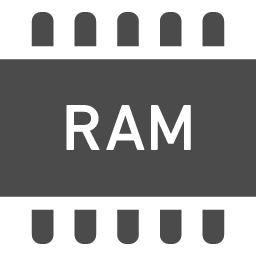
\includegraphics[height=8mm]{figs/assets/memory.png}\\ \textbf{OOM} ${\approx}20$\,GB / $24$\,GB};
  \node[t, below right=12mm and -10mm of wrap] (npq) {
\includegraphics[height=8mm]{figs/assets/shield.png}\\ \textbf{not post-quantum} (pairing-based)};
  \draw[->] (root) -- (bare);
  \draw[->] (root) -- (wrap);
  \draw[->] (bare) -- (noanon);
  \draw[->] (wrap) -- (oom);
  \draw[->] (wrap) -- (npq);
\end{tikzpicture}
\caption{The dual obstruction. The proof feasible to generate (left, the bare STARK
receipt) is not zero-knowledge, hence not anonymous; the proof that would be
zero-knowledge (right, a Groth16/PLONK wrap) is blocked by two \emph{independent}
prongs: resource (OOM at ${\approx}20$~GB) and primitive (pairing-based, not
post-quantum, which more memory cannot fix). Solid edges mark a produced step, dashed
a blocked one.}
\label{fig:dual-obstruction}
\end{figure}

BDEC's anonymity and unlinkability require the underlying argument to be
zero-knowledge. The succinct STARK receipt produced by either zkVM is, in the
configurations we run, an argument of knowledge but not a zero-knowledge one, and
this holds on both substrates for separately documented reasons. SP1's
specification states plainly that its STARK proofs are not
zero-knowledge~\cite{sp1docs-sec}. RISC~Zero documents perfect zero-knowledgeness
for its STARK, but independent analysis by Habock and Al~Kindi, together with
RISC~Zero's own security advisory, finds that several STARK implementations,
RISC~Zero among them, do not provably meet the zero-knowledge
requirement~\cite{risc0zkadvisory,l2beatzk}. We therefore treat the bare receipt
as not dependably zero-knowledge on either substrate, a concrete instance of the
caution that a system may be called a zkVM without delivering zero-knowledge.
Zero-knowledge is obtained only by wrapping the receipt in a succinct proof, and
the wraps SP1 exposes, Groth16 and PLONK, are pairing-based and therefore only
classically secure. The barrier splits into two independent obstructions, set out
below. Both block anonymity for separate reasons, and naming each one precisely
is the security-level result of this analysis.

The first obstruction is one of resources. On the target hardware at
$\lambda=80$ the PLONK wrap exhausts memory at ${\approx}20$~GB on the $24$~GB
machine (killed under memory pressure; Section~\ref{sec:evaluation}), so the
anonymity-providing proof is infeasible to generate even though the bare,
non-anonymous receipt is. The second obstruction
is one of primitives. Even with unlimited memory, wrapping a post-quantum STARK
receipt in a pairing-based Groth16 or PLONK proof re-introduces a
quantum-vulnerable assumption into the anonymity guarantee, the very class of
assumption the post-quantum motivation rules out (Section~\ref{sec:related}).
Such a wrap remains acceptable for a classically-secure deployment, and Groth16
and PLONK are not unsuitable in general. They are ruled out here only by the
thesis's post-quantum-anonymity goal.
Recovering post-quantum anonymity requires a post-quantum-sound zero-knowledge
wrap, for instance a STARK-based or lattice-based recursive argument, which the
deployed toolchains do not yet provide.

We therefore use the classically secure Groth16 or PLONK wrap to locate the
resource cost. It is not a deployable post-quantum-anonymous configuration. The
two obstructions together leave no good option on commodity hardware: the proof
that is feasible to generate is not anonymous, and the proof that would be
anonymous is neither feasible to generate nor, with the available wraps,
post-quantum. Within the scope of the
literature we surveyed, we did not find this conjunction stated explicitly for
post-quantum anonymous credentials, and surfacing it is a contribution of this thesis: we
quantify the resource prong, the $24$~GB wrap frontier of
Section~\ref{sec:evaluation}, and identify the primitive prong as a toolchain
gap.

The barrier is scoped to the substrate and hardware studied: an Apple M5~Pro with
$24$~GB of memory, the CPU-bound provers of RISC~Zero and SP1, and the parameter
set $\lambda=80$. We do not claim the barrier is fundamental to the primitive or
that it persists on server-class hardware. Characterising how it moves with the
memory budget and the security level is left to Section~\ref{sec:conclusion}.
